\documentclass[12pt,letterpaper]{article}
\usepackage{forest}
\title{HW4}
\author{ZONGQI CUI}
\begin{document}
\maketitle
    \section{Assignment 4-1}
        \begin{center}
        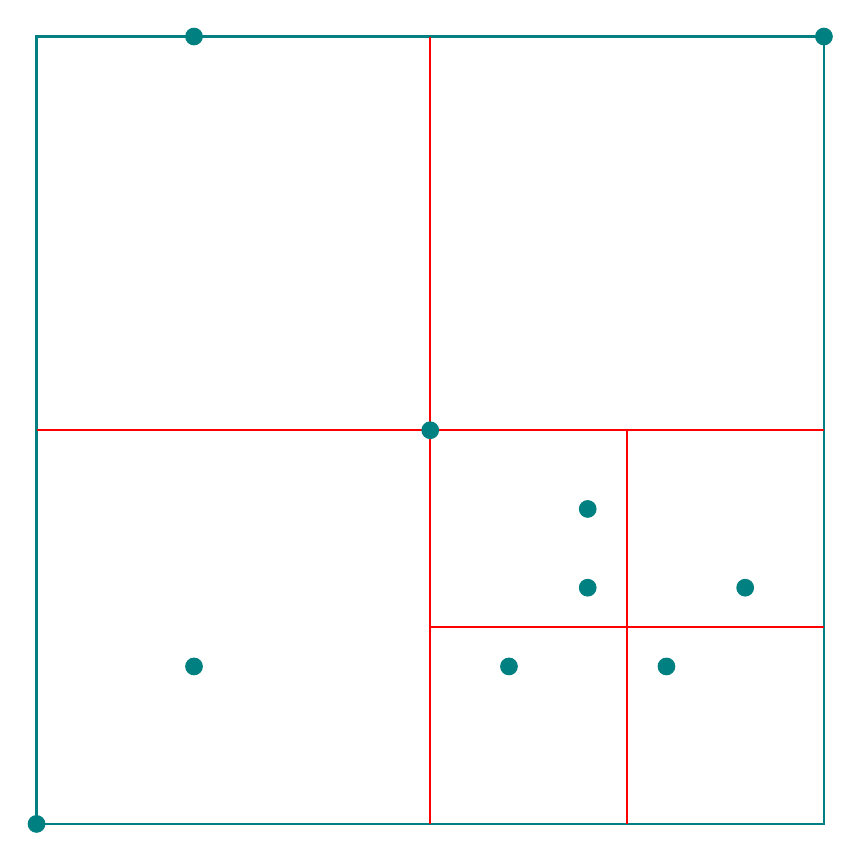
\begin{tikzpicture}
        
        \draw[thick, teal] (0,0) rectangle (10,10);
        
        % Draw the splits (red lines)
        \draw[thick, red] (5,0) -- (5,10);  % Vertical split
        \draw[thick, red] (0,5) -- (10,5);  % Horizontal split
        \draw[thick, red] (7.5,0) -- (7.5,5); 
        \draw[thick, red] (5,2.5) -- (10,2.5); 
        
        
        \filldraw[teal] (0,0) circle (3pt); % Point A
        \filldraw[teal] (10,10) circle (3pt); % Point B
        \filldraw[teal] (8,2) circle (3pt); % Point C
        \filldraw[teal] (9,3) circle (3pt); % Point D
        \filldraw[teal] (2,2) circle (3pt); % Point E
        \filldraw[teal] (6,2) circle (3pt); % Point F
        \filldraw[teal] (2,10) circle (3pt); % Point G
        \filldraw[teal] (7,3) circle (3pt); % Point H
        \filldraw[teal] (5,5) circle (3pt); % Point I
        \filldraw[teal] (7,4) circle (3pt); % Point J
        
        \end{tikzpicture}
        \end{center}
    
    \section{Assignment 4-2}
        \begin{center}
        \begin{tikzpicture}
        
        \draw[thick, teal] (0,0) rectangle (10,10);
        
        
        \draw[thick, red] (7.9,0) -- (7.9,10); 
        \draw[thick, red] (7.9,2.1) -- (0,2.1); 
        
        \filldraw[teal] (0,0) circle (3pt); % Point A
        \filldraw[teal] (10,10) circle (3pt); % Point B
        \filldraw[teal] (8,2) circle (3pt); % Point C
        \filldraw[teal] (9,3) circle (3pt); % Point D
        \filldraw[teal] (2,2) circle (3pt); % Point E
        \filldraw[teal] (6,2) circle (3pt); % Point F
        \filldraw[teal] (2,10) circle (3pt); % Point G
        \filldraw[teal] (7,3) circle (3pt); % Point H
        \filldraw[teal] (5,5) circle (3pt); % Point I
        \filldraw[teal] (7,4) circle (3pt); % Point J
        
        \end{tikzpicture}
        \end{center}
        
\end{document}